
One of the hurdles with most state-of-the-art open source topology optimization tools is their input format, where many of them (including ToPy, our topology optimizer of choice) require input to be specified as a 3-dimensional voxel grid. Presence (or absence) of material in these voxels is defined by a boolean variable, and boundary conditions are imposed on the appropriate locations. An example of voxelized data can be seen in \autoref{fig: voxelOpenCascade}. %Since there is a variety of toolboxes available which are able to perform a voxelization of common CAD input files, we did not implement one of our own but rather adapted one of the open source tools. %This section describes how we overcame this hurdle of converting CAD representations to voxelized input.
\begin{figure}
\centering
  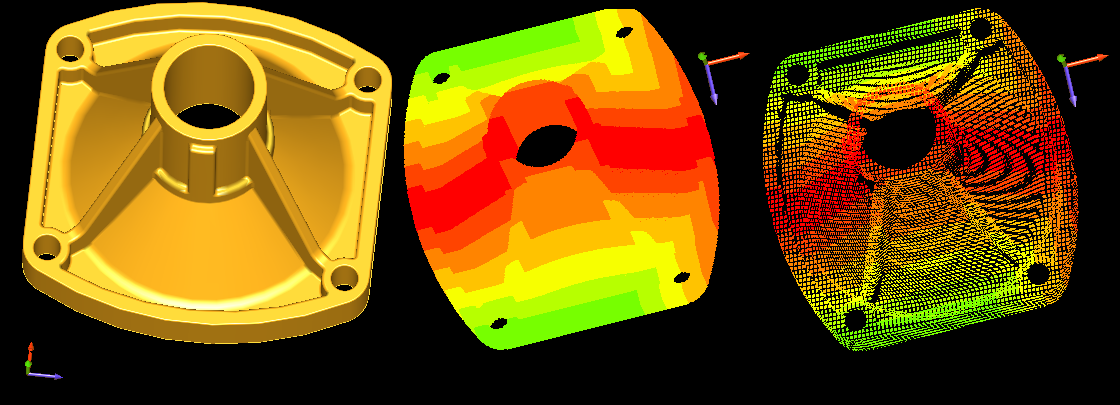
\includegraphics[scale=0.3]{Pictures/CADToVoxel/voxels_wp_image005.png}
\caption{A shape and its voxel representation. \emph{Leftmost picture}: The original parametrized shape. \emph{Rightmost picture}: The voxel representation. Picture from OpenCascade \cite{OpenCascade}.}
\label{fig: voxelOpenCascade}
\end{figure}

\label{sec:CVMLCPP}
In the variety of toolboxes available for voxelization, we decided on the \emph{Common Versatile Multi-purpose Library for C++} (CVMLCPP). This is a collection of mathematical algorithms whose objective is "to eliminate this redundancy by offering high-quality implementations of commonly needed functionality" \cite{CVMLCPP}. The library offers an easy-to-use voxelizer, which we use for conversion of CAD input to a boolean voxel grid.

Another very popular open-source choice is the 3D modeling toolbox is OpenCascade \cite{OpenCascade}, a versatile library with huge amounts of functionality. Although this also offers a voxelizer, we decided that its additional functionality did not justify its disadvantages in size and cumbersome installation requirements on for example a linux system.
\begin{figure}
\centering
\begin{subfigure}{
  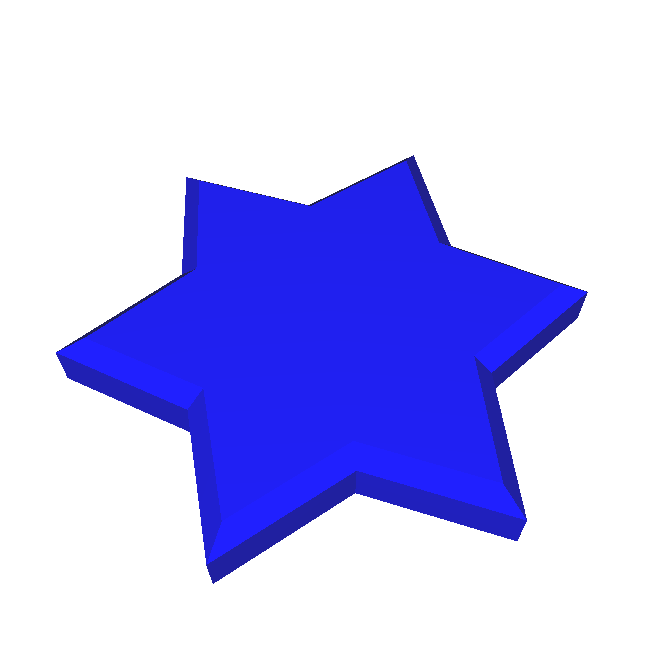
\includegraphics[width=.2\linewidth]{Pictures/STLToVoxels/Star_STL.png}}
\end{subfigure}
\begin{subfigure}{
  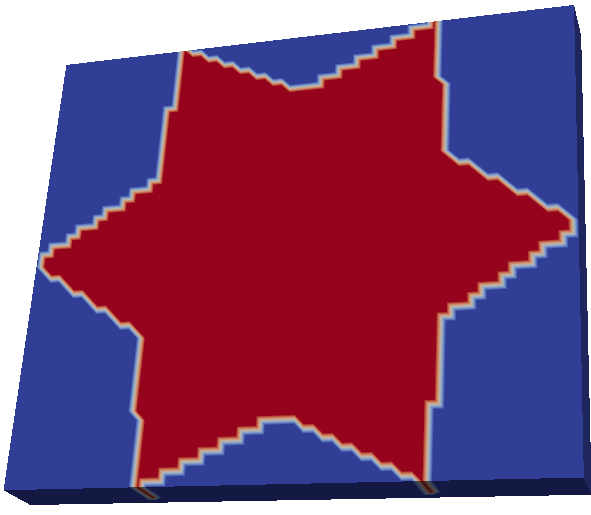
\includegraphics[width=.2\linewidth]{Pictures/STLToVoxels/Star_VTK_Trans.png}}
\end{subfigure}
\caption{The STL geometry of a star (left) and its voxelized form (right) obtained via the CVMLCPP voxelizer, visualized by Paraview \cite{Paraview}.}
\label{fig: voxelizerStar}
\end{figure}

In terms of implementation, the only thing required is the installation of the CVMLCPP library. The voxelizer is then included as a callable binary, that takes STL-file input (\autoref{subsub:STL}) and converts it to a .dat binary file with dimension and voxel information, with specifiable voxel size. An example result of using the voxelizer is shown in \autoref{fig: voxelizerStar}.
 %In the end, to voxelize a file given as .stl-input, we could just call 
%\begin{lstlisting}
%~/Path/To/CVMLCPP/bin/voxelize ./<stl_file>.stl <voxelSize>
%\end{lstlisting}
%where $\mathtt{<voxelSize>}$ is an integer declaring the size of a voxel. 
